% Results
%
%	some important things to know
% 	experimental parts in the chapter results
%	numerical results or so-called data
%	order of presentation
% 	cross references

\chapter{Results}

\section{Implemented System}

The implemented system consist of tree pieces of software. The software controlling the acquisition card in the machine. An acquisition software that run on a normal front-end Linux machine that is taking data during the \glspl{MD}. And an analyzing software. The analyzing software is in fact modular and has a version that has to run on a GPU enable machine to use the GPU to compute the \glspl{FFT}.

\begin{figure}[H]
\caption{Implemented acquisition software in the CERN infrastructure}
\centering
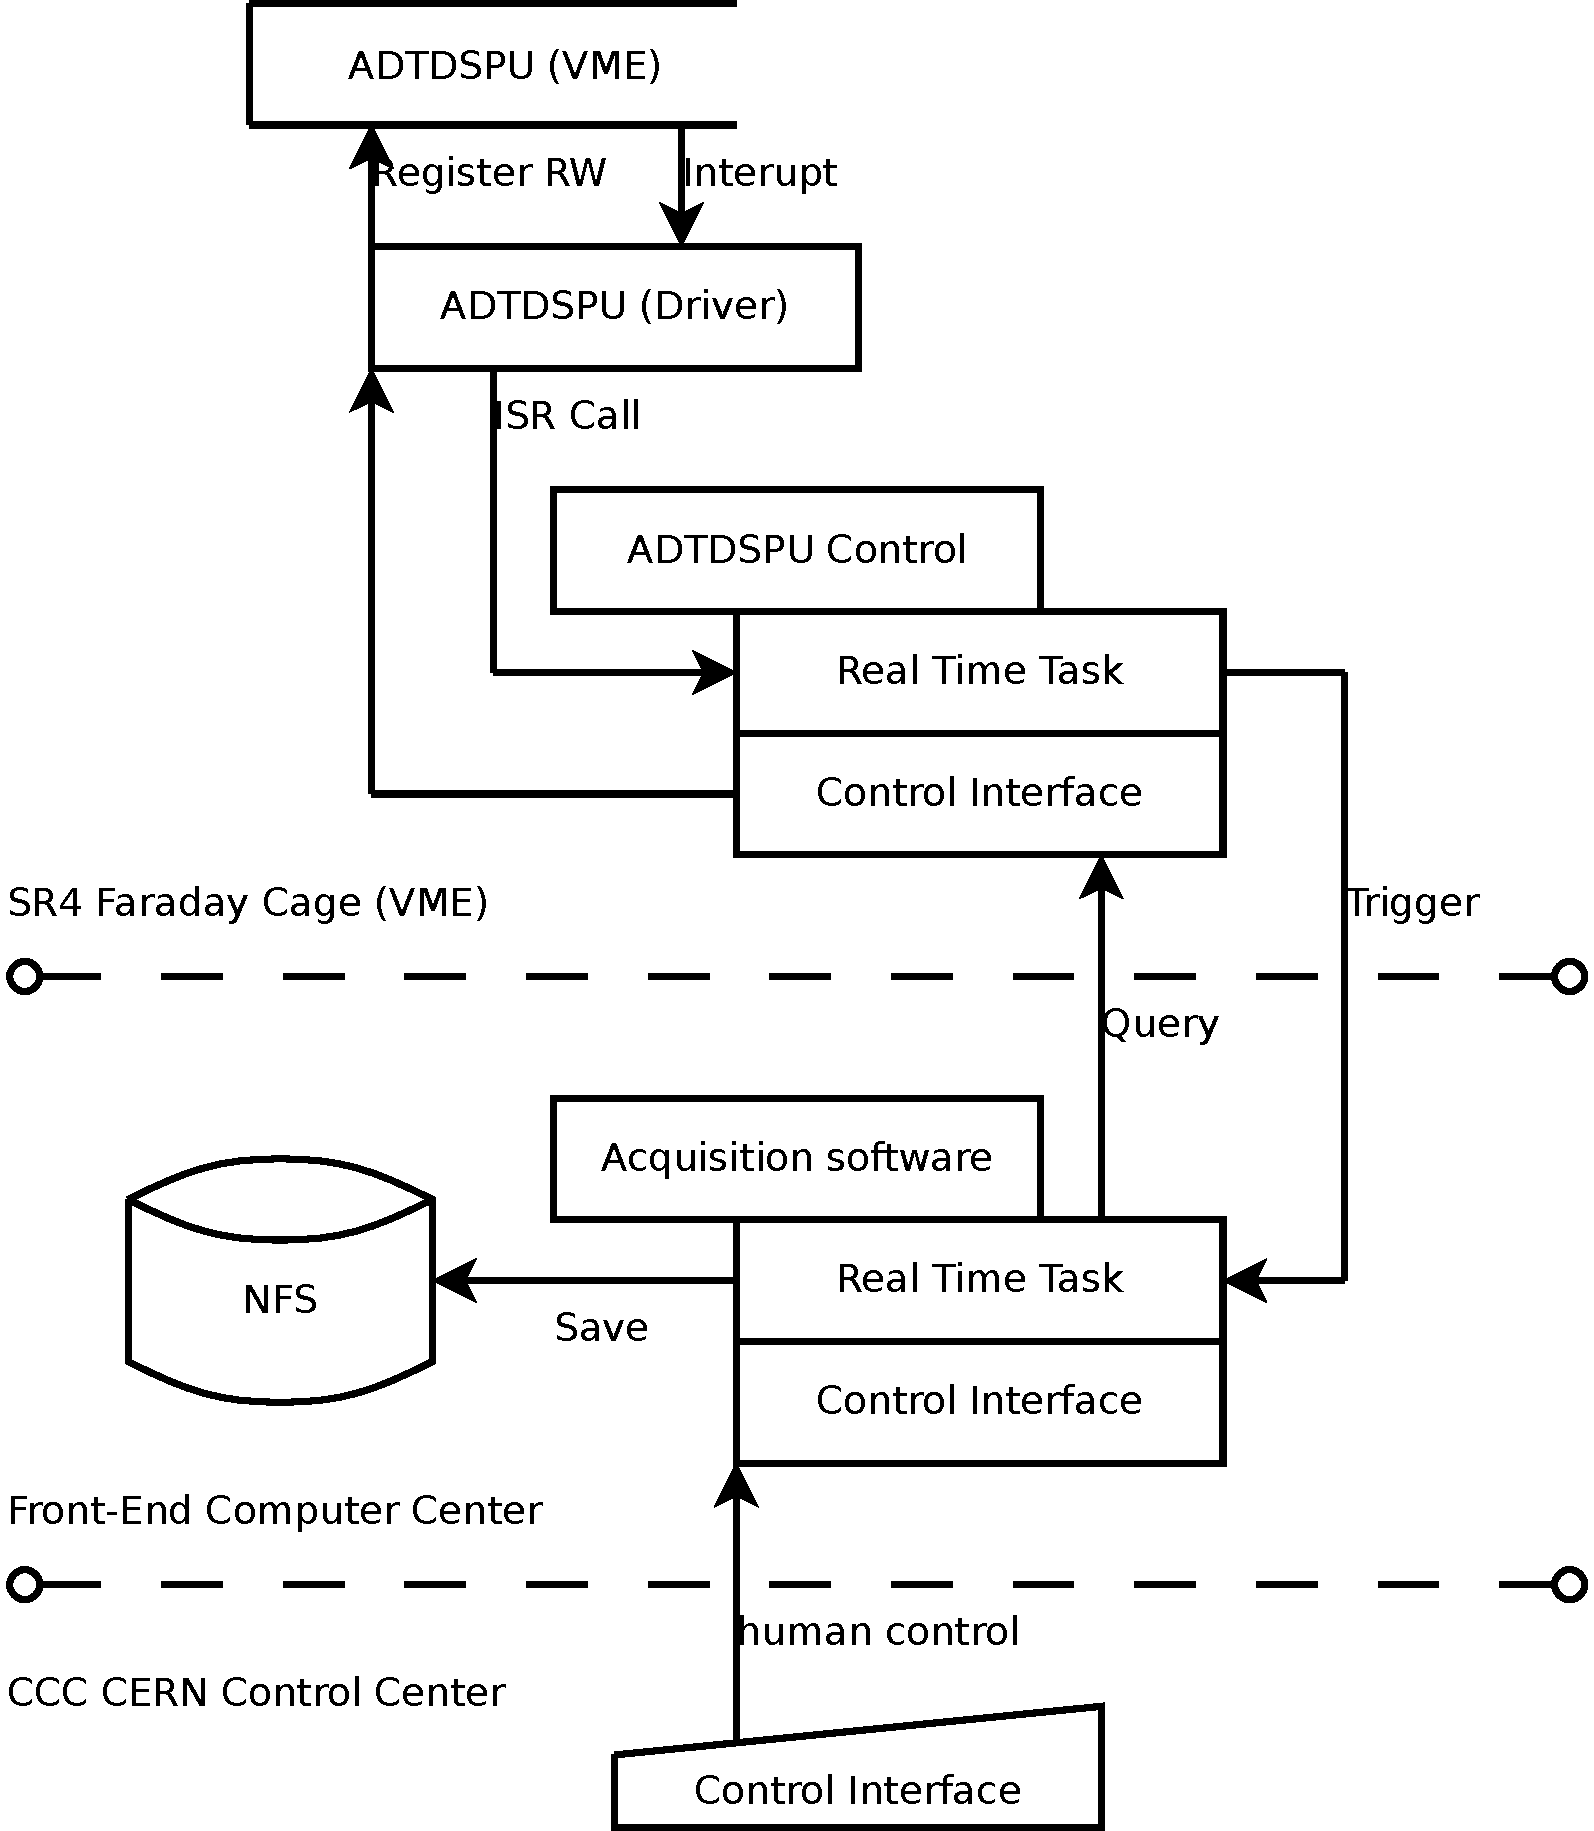
\includegraphics[scale=0.3]{ImplementedSoftFesa.pdf}
\end{figure}

In the final version the software will be merged in single executable that should run on the \gls{GPU}-enabled machine. This solution has been put into place because the present hardware is still in development and there is no way of acquiring the full 2880 bunches of the machine, the hardware is receiving the acquisition data but the \gls{VME} is not fast enough to transfer it to the \gls{CPU}.

	\subsection{ADTDSPU control software}

	The first layer that was needed is a driver that can control the \gls{VME} card and forward the interrupts. This is using standard driver framework from the \gls{CO} group at \gls{CERN}.

	Then the normal \gls{FESA} environment is used to develop a higher level software to control the card. This particular card need real time task to react to interrupt coming from the hardware to inform when new acquisition is ready to be read.

	\subsection{Acquisition software}

	The acquisition software was used to check that the idea of getting the tune out of the DSPU card was doable and being able to log the acquisition to file to be checked and processed separately.

	It uses \gls{CMW}, a library used at \gls{CERN} to communicate between different layers of the accelerators control software, to connect to the the ADTDPSU control software and get the data when they are published (at interrupt time).

	It is then able to compute the acquisition \gls{FFT} using \gls{FFTW} and display it to the operators in the \gls{CCC} where all the eight accelerators of \gls{CERN} are controlled. On the interface you can decide witch type of graph you want to see and also enable saving the data into files to be processed by the data analysis software.

	\subsection{Data analysis software}

	The data analysis software is a set of modules that can be enabled or bypassed to test the the usefulness of an algorithm. As we have precise time allocated to make the full computation this allow to test the different modules.

	The data is first loaded from the files that were written by the acquisition software. Then it is filtered by a notch filter as described in the notch section~\ref{sec:notch}. And finally to the different algorithms as shown in the figure~\ref{fig:PCFlow}.

	First optional step is \gls{SVD} this as described in Rama Calaga PHD thesis\cite{calaga06} and Wolfgang H{\"o}fle\cite{HofleChamonix12} should reduce noise in the signal result are seen in section\ref{sec:SVD}.

	Then come the the \gls{FFT} either using the \gls{GPU} or using the \gls{CPU}, actually you could use \gls{OpenCL} on the \gls{CPU} and test the whole \gls{OpenCL} path. The different path are due to memory copying, in the case of computation made on the \gls{GPU} you have to move the memory data from the \gls{CPU} central memory to the \gls{GPU} memory. this will described in section~\ref{sec:FFT}.

	To have a clear image and to combine the real and imaginary part of the \gls{FFT} we use the amplitude. It has been validated in the acquisition software as been the best metric, this could be changed as will in the final version. The amplitude is described in section~\ref{sec:amplitude}.

	As a final value is wanted we do the accumulation of all the bunches, it will give an average spectrum of the whole machine.

	The normalization step is just present for displaying the spectrogram (see section~\ref{sec:spectrogram}) and will not be needed for the final version.
 
	\begin{figure}[h]
	\caption{Time flow with different implementations and with 3000 bunches of 
	2048 points each.}
	\centering
	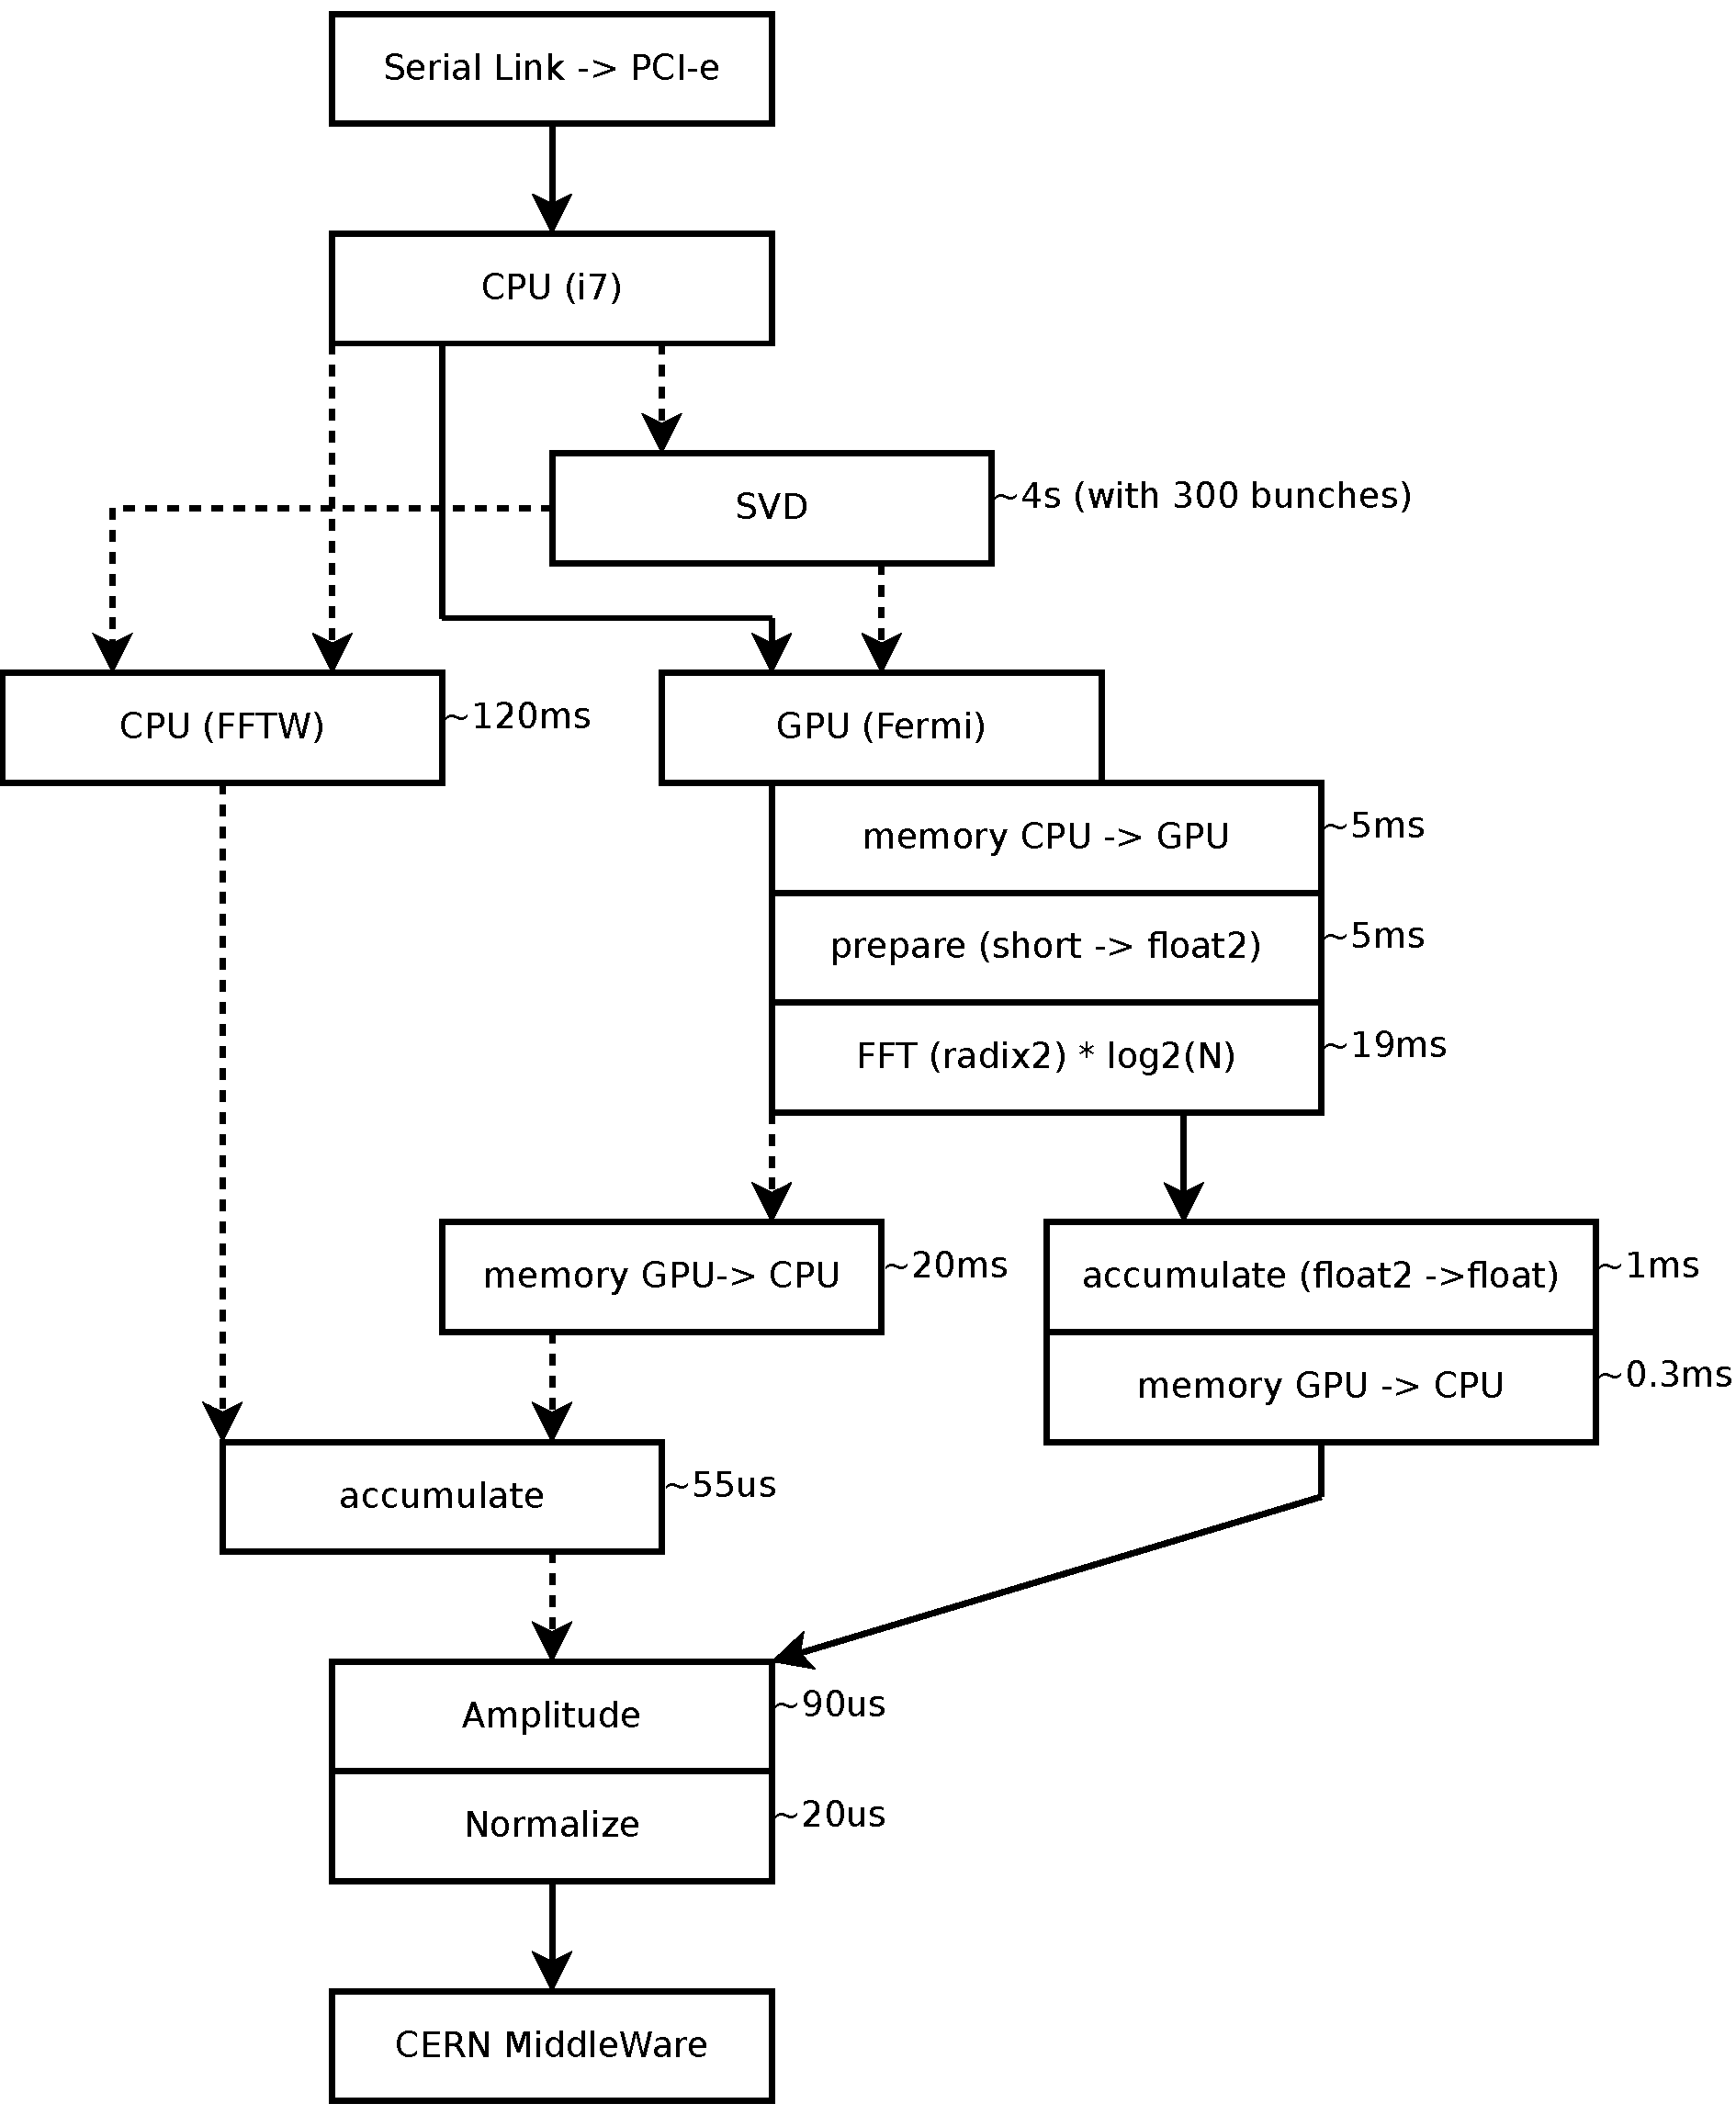
\includegraphics[scale=0.3]{PC-flow.pdf}
	\label{fig:PCFlow}
	\end{figure}

\section{Notch filter}
\label{sec:notch}

A notch filter is used to cut the low frequencies, this doesn't change anything on the high frequencies, it won't be used in the final version. For every sample it takes the present sample and subtract the next element.

$$y_{[n]} = x_{[n]} - x_{[n + 1]}$$

This is a differential filter, as we are only interested into the higher frequency this has no incidence on our results and allow for a better visualization of the spectrograms.

\section{FFT}
\label{sec:FFT}

The Fourier transform is a mathematical operation that moves a function from a temporal domain to a frequency domain. In our case we are talking about \gls{DFT}, and in particular, the \gls{FFT}.

	\subsection{Definition}

	The \gls{DFT} is a discrete transform. It transform a function into another, which is called frequency domain, or simply \gls{DFT}, of the original function.

	$$ x_0,...,x_{N -1} \in \mathbb{C} $$

	$$ X_{k} = \displaystyle\sum\limits_{n = 0}^{N -1} x_{n}e^{-i 2 \pi k \frac{n}{N}} $$

	In order to compute the \gls{DFT} one must compute N number of values N times. The complexity is thus

	$$ \mathcal{O}(N^{2}) $$

	The most commonly used \gls{FFT} algorithms are based on a divide-and-conquer approach similar to the algorithm of Cooley and Turkey\cite{Cooley65}. The computation of a \gls{DFT} of length N is done by splitting the input sequence into a fixed small number of subsequences, compute their \gls{DFT}, and assemble the outputs to build the final sequence. If the split and assembly are linear in time the complexity becomes 

	$$ \mathcal{O}(N \log(N)) $$

   \subsection{FFTW}

   Some words that explain what is FFTW and why is was chosen as a reference

   \subsection{FFT with OpenCL on GPU}

   Some words on the implementation used for calculating FFT on OpenCL reference to the image of the spectrogram.

   \subsection{FFT with OpenCL on CPU}

   Some words on the fact that you can run the code on the CPU as well and then reference on the figure.

   Also talk about the fact that there is less noise in the OpenCL CPU version than the OpenCL GPU version.

\section{Amplitude}
\label{sec:amplitude}

Amplitude calculation formula, explain the figures tell why it has to be done before accumulation and show this is very fast reference to the table of perf.

\section{SVD}
\label{sec:SVD}

Problem is not directly solvable with the number of bunch observed cite H{\"o}fle and Rama need a lot more bunches to make a good smooth\cite{calaga06}. 

Talk about the performances issues and cite the paper on SVD on GPU as a future implementation (could go to discussion?)\cite{Lahabar09}

\section{Performances}

Calculation made by accumulation to simulate the number of bunches that could be present in the final version (2880).

   \subsection{Pipelining}

	Pipelining was tested and used in the process and it was possible to win around 10\% in performances around it.

   \subsection{Memory}

	Copy of memory from and to the GPU discution.

   \subsection{Time}

	Add table with time performances and discution.

	\begin{table}[H]
		\caption{Speed for 3000 batch of 2048 points}
		\begin{tabular}{|l|lrrcr|}
			\hline
				Device & Type & Threads & Speed [GHz] & pipeline & Time [ms] \\
			\hline
			\hline
				Xeon X5650 & FFTW & 12 & 2.67 & N/A & 291 \\
				Xeon X5650 & OpenCL & 12 & 2.67 & enable & 284 \\
				Xeon X5650 & OpenCL & 12 & 2.67 & disable & 288 \\
			\hline
				i7-3720QM & FFTW & 8 & 2.6 & N/A & 310 \\
				i7-3720QM & OpenCL & 8 & 2.6 & enable & 272 \\
				i7-3720QM & OpenCL & 8 & 2.6 & disable & 273 \\
			\hline
			\hline
				Tesla M2090 & OpenCL & 512 & 1.3 & enable & 35 \\
				Tesla M2090 & OpenCL & 512 & 1.3 & disable & 37 \\
			\hline
				GeForce 650M & OpenCL & 384 & 0.9 & enable & 355 \\
				GeForce 650M & OpenCL & 384 & 0.9 & disable & 365 \\
			\hline
		\end{tabular}
	\end{table}

\section{Spectrogram}
\label{sec:spectrogram}

Some word definition of Spectrogram. Display some spectrogram.

\begin{figure}[H]
	\caption{Spectrogram with ADT off on the 16 October 2012 on vertical beam 1 during squeeze and collision}
	\centering
	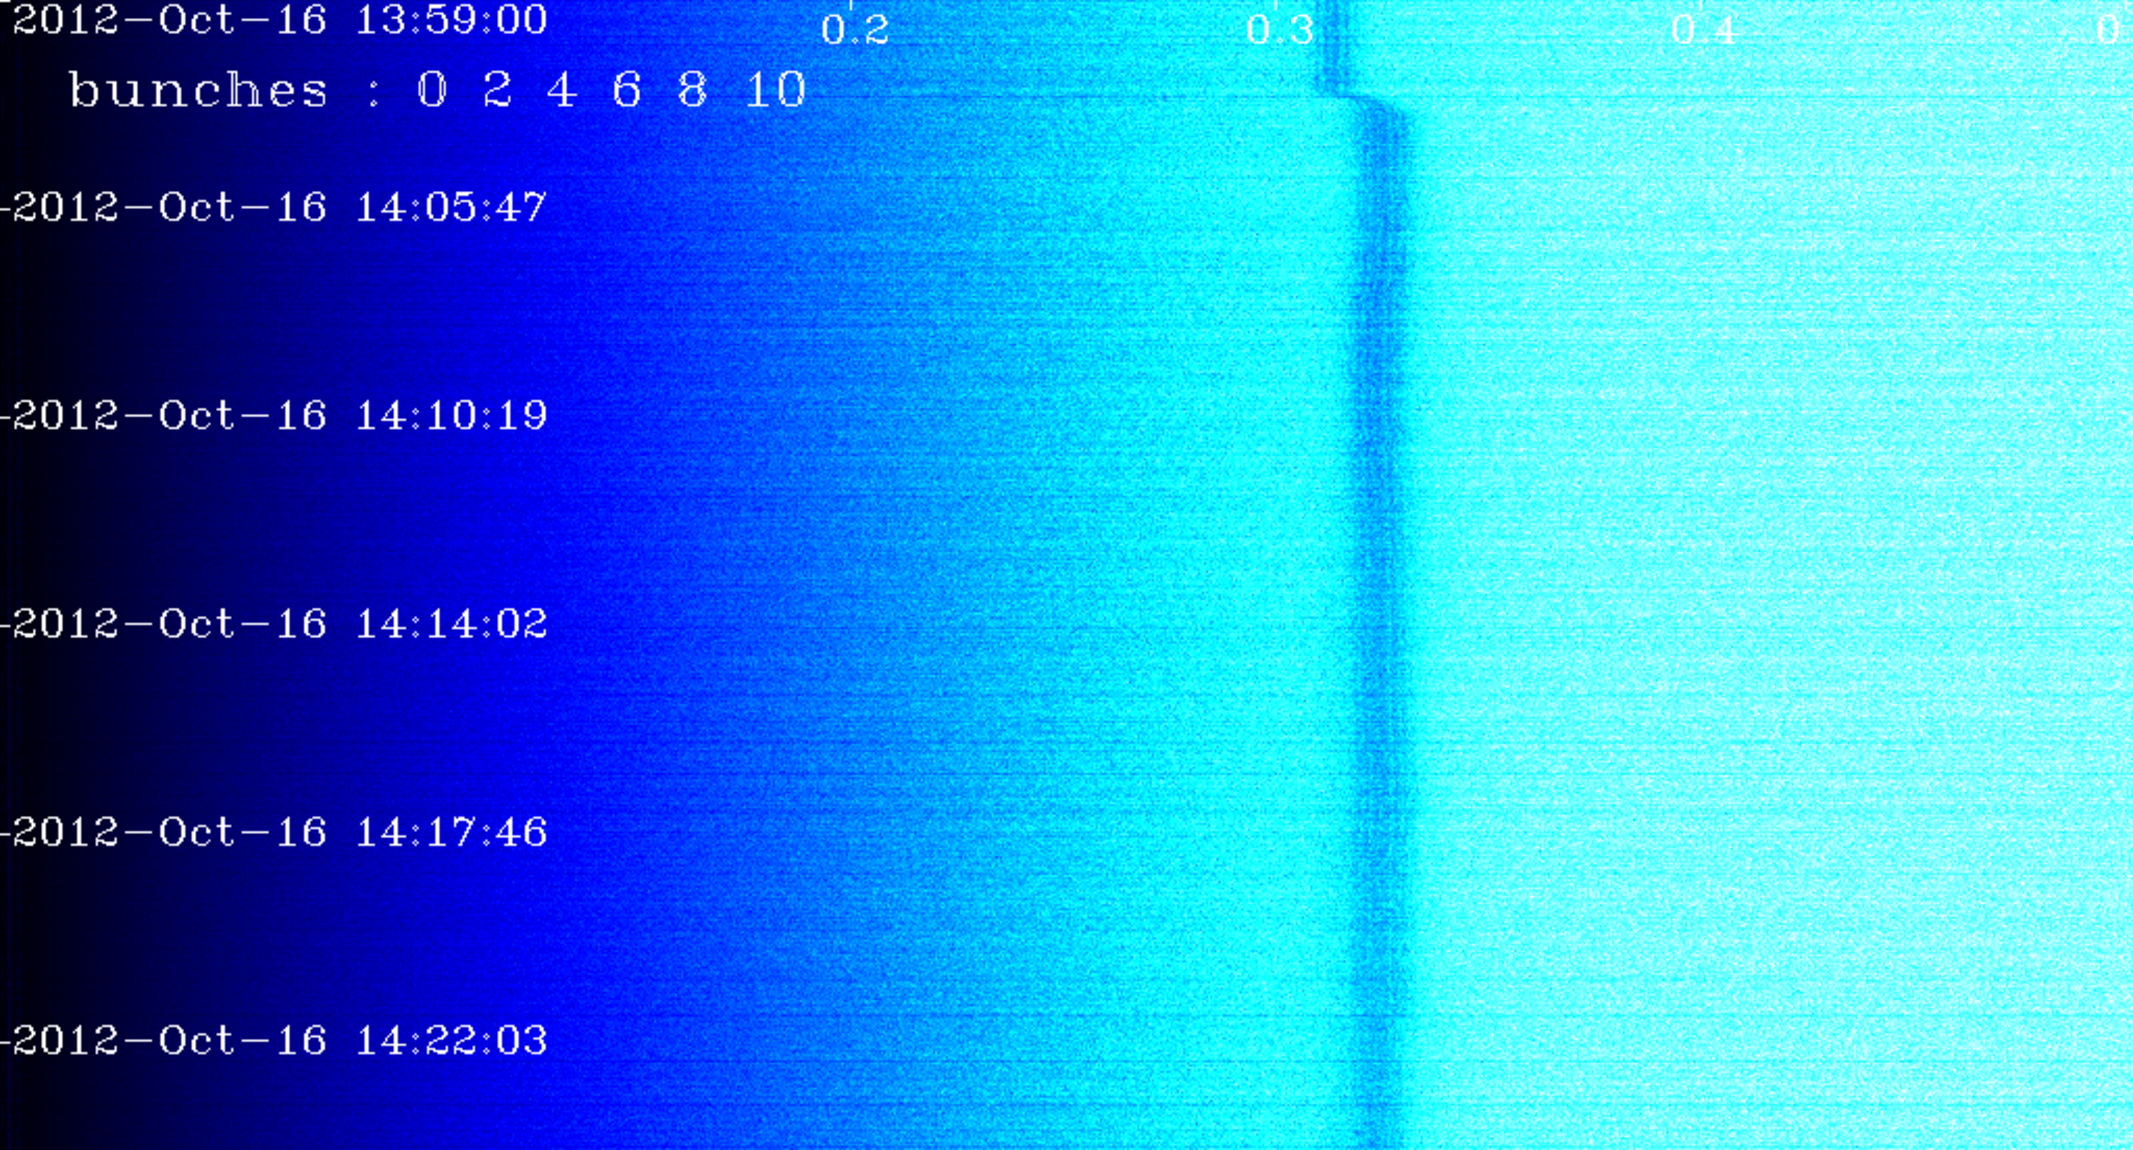
\includegraphics[scale=0.3]{md-121016-vb1-m1-6bunches-10acc-1359-1425-collision.pdf}
\end{figure}